\chapter{Tecnologias \textit{Web}}

\section{\textit{Framework}}
Segundo \citeonline{artigo_oo_reuso_software}, a programação orientada a objetos é muita vezes utilizada para promover o reuso de software. Para \citeonline{artigo_reuso_classes}, algumas linguagens, como \textit{Smalltalk}, são utilizadas tanto para reduzir o tempo de desenvolvimento quanto o custo de manutenção, simplificando a criação de novos sistemas e de novas versões para sistemas já existentes. Afirma, também, que ``componentes de um programa devem ser projetados para reusabilidade''.

Os mesmos autores confirmam que um ``design abstrato orientado a objetos'', também chamado de \textit{framework}, define uma interface para os principais componentes dentro de uma
arquitetura pré-definida. ``\textit{Frameworks} provêem uma maneira de reutilizar código que é resistente a mais tentativas de reusos convencionais''.

\citeonline{artigo_reuso_classes}, comparam ``programas esqueletos'' com \textit{frameworks}, os quais consistem em uma abordagem tradicional de reutilização de código e na garantia de consistência entre todos os componentes de um sistema sobre a mudança de algum requisito. O autor também realiza uma comparação entre os \textit{frameworks} do tipo ``caixa-branca'' e ``caixa-preta'', o primeiro é responsável por especificar o comportamento de uma aplicação adicionando-se métodos para subclasses de uma ou mais de suas classes, ou seja, a implementação deste tipo de \textit{framework} deve ser conhecida para sua utilização, o segundo consiste no uso de um protocolo responsável por definir uma interface entre os componentes,. Deste modo, o usuário precisaria entender apenas como funciona a interface externa dos componentes para utilizá-los.

\section{Ferramentas \textit{Web} Utilizadas}
    \subsection{\textit{Coverage}}
    Coverage\footnote{\url{https://pypi.python.org/pypi/coverage/}} é uma ferramenta python responsável por medir a cobertura de código para o conjunto de testes unitários utilizado. A ferramentas rastreia quais linhas de código foram executadas pela suíte de testes.

    \subsection{\textit{GitLab CI}}
    \textit{GitLab CI}\footnote{\url{https://about.gitlab.com/gitlab-ci/}} ferramenta integrada ao {GitLab} para realizar serviços de integração contínua a cada \textit{commit}. A integração contínua está configurada para instalar as dependências do projeto, executar a suíte de testes e verificação de estilo com flake8\footnote{url{https://pypi.python.org/pypi/flake8}}.

    \subsection{\textit{Django-Cron}}
    \textit{Django-Cron}\footnote{\url{http://django-cron.readthedocs.io/en/latest/index.html}} é uma ferramenta para execução de \textit{scripts} em \textit{python} de forma temporizada.

    \subsection{\textit{Sphinx}}
    \textit{Sphinx}\footnote{\url{http://www.sphinx-doc.org/}} é uma ferramenta para criação inteligente e estilizada de documentação de códigos em \textit{python}, C/C++
    e outras linguagens. Utiliza \textit{reStructuredText}\footnote{\url{http://docutils.sourceforge.net/rst.html}} como sua linguagem de marcação e converte toda a documentação para formato html, pdf, epub ou man.

\section{Protocolos Utilizados}    

    \subsection{UDP}
    O protocolo UDP (\textit{User Datagram Protocol}, Protocolo de Datagrama do Usuário) é um protocolo da camada de transporte e não orientado a conexões. Seu cabeçalho, figura \ref{udp_header}, possui 8 \textit{bytes}, seguido de uma carga útil. As portas apresentadas no cabeçalho representam as máquinas de origem e destino \cite{tanenbaum_2002}.

    \begin{figure}[!htpb]
        \centering
        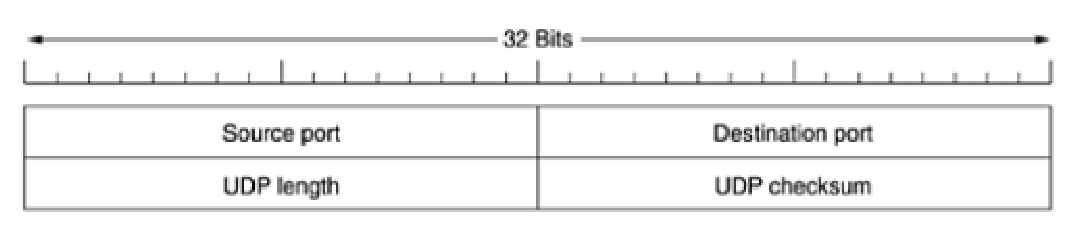
\includegraphics[keepaspectratio=true,scale=0.8]{figuras/udp_header.eps}
        \caption{Cabeçalho do UDP. Fonte: \cite{tanenbaum_2002}}
        \label{udp_header}
    \end{figure}

    O protocolo \textit{Modbus RTU} é encapsulado no campo de dados do protocolo UDP. Neste encapsulamento, o endereço ModBus de todos os equipamentos é igual a 1, sendo que a diferenciação entre equipamentos se dá pelo número de IP.